\chapter{Arquitectura del Dashboard}

\section{Diseño Arquitectónico}
El dashboard PLANEA fue diseñado con una arquitectura modular y flexible que permite la integración eficiente de múltiples componentes y facilita el mantenimiento y la escalabilidad.

\subsection{Principios de Diseño}
El diseño arquitectónico se basó en los siguientes principios:

\begin{itemize}
    \item \textbf{Modularidad}: Organización en componentes independientes y reutilizables.
    \item \textbf{Separación de preocupaciones}: Clara distinción entre lógica de procesamiento de datos, visualización y control de la interfaz.
    \item \textbf{Escalabilidad}: Capacidad para incorporar nuevos datos, métricas o visualizaciones.
    \item \textbf{Mantenibilidad}: Facilidad para actualizar y corregir componentes individuales sin afectar al conjunto.
    \item \textbf{Rendimiento}: Optimización para manejar eficientemente grandes volúmenes de datos.
\end{itemize}

\subsection{Estructura General}
La arquitectura del dashboard se organiza en tres capas principales:

\begin{figure}[h]
    \centering
    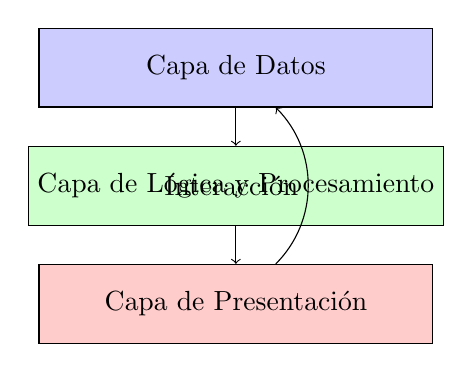
\begin{tikzpicture}[node distance=1.5cm]
        \node (datos) [rectangle, draw, fill=blue!20, minimum width=5cm, minimum height=1cm] {Capa de Datos};
        \node (logica) [rectangle, draw, fill=green!20, minimum width=5cm, minimum height=1cm, below of=datos] {Capa de Lógica y Procesamiento};
        \node (present) [rectangle, draw, fill=red!20, minimum width=5cm, minimum height=1cm, below of=logica] {Capa de Presentación};
        
        \draw[->] (datos) -- (logica);
        \draw[->] (logica) -- (present);
        \draw[->] (present) to [bend right=45] node[left] {Interacción} (datos);
    \end{tikzpicture}
    \caption{Arquitectura en tres capas del dashboard PLANEA}
    \label{fig:arquitectura}
\end{figure}

\begin{itemize}
    \item \textbf{Capa de Datos}: Gestiona la carga, almacenamiento y acceso a los datos de PLANEA.
    \item \textbf{Capa de Lógica y Procesamiento}: Implementa los algoritmos, cálculos y transformaciones necesarios.
    \item \textbf{Capa de Presentación}: Maneja la interfaz de usuario y las visualizaciones.
\end{itemize}

\section{Organización de Ficheros}
El sistema está organizado en un conjunto de ficheros Python que implementan diferentes aspectos de la funcionalidad.

\subsection{Estructura de Ficheros}
La estructura principal de ficheros es la siguiente:

\begin{lstlisting}[caption=Estructura de ficheros del dashboard]
DASHBOARD PLANEA/
|-- dashboard_completo.py         # Archivo principal
|-- utils.py                      # Utilidades y funciones comunes
|-- dashboard_completo_tab1.py    # Implementación de KPIs Principales
|-- dashboard_completo_tab2.py    # Análisis por Año (2015-2017)
|-- dashboard_completo_tab3.py    # Análisis por Estado
|-- dashboard_completo_tab4.py    # Datos 2022
|-- dashboard_completo_tab5.py    # Tablas y Estadísticas
|-- DATOS2015-2017.xlsx           # Datos fuente 2015-2017
|-- DATOS2022.xlsx                # Datos fuente 2022
\end{lstlisting}

\subsection{Descripción de Componentes Principales}
\begin{itemize}
    \item \textbf{dashboard\_completo.py}: Archivo principal que coordina la carga de datos y la integración de las diferentes pestañas.
    \item \textbf{utils.py}: Contiene funciones de utilidad reutilizables, como normalización de columnas y cálculo de métricas.
    \item \textbf{dashboard\_completo\_tabN.py}: Implementación específica de cada pestaña, con sus visualizaciones y análisis particulares.
\end{itemize}

\section{Gestión de Datos}

\subsection{Estrategia de Carga}
La carga de datos se implementa en el archivo principal con un enfoque que prioriza la eficiencia y la flexibilidad:

\begin{lstlisting}[language=Python, caption=Implementación de carga de datos]
@st.cache_data
def cargar_datos(archivo, anio, max_rows=None):
    try:
        if archivo == "DATOS2015-2017.xlsx":
            df = pd.read_excel(archivo, sheet_name=f"{anio}")
        else:
            df = pd.read_excel(archivo)
        
        if max_rows:
            df = df.head(max_rows)
            
        return normalizar_columnas(df)
    except Exception as e:
        st.error(f"Error al cargar datos de {anio}: {str(e)}")
        return None
\end{lstlisting}

Características clave:
\begin{itemize}
    \item \textbf{Uso de caché}: Mediante el decorador \texttt{@st.cache\_data} para evitar recargas innecesarias.
    \item \textbf{Control de volumen}: Parámetro \texttt{max\_rows} para limitar la cantidad de datos cargados.
    \item \textbf{Manejo de errores}: Captura y presentación de errores sin interrumpir la ejecución.
    \item \textbf{Normalización integrada}: Aplicación automática de la normalización de columnas.
\end{itemize}

\subsection{Flujo de Datos}
El flujo de datos a través del sistema sigue el siguiente patrón:

\begin{enumerate}
    \item \textbf{Carga inicial}: Los datos se cargan desde los archivos Excel.
    \item \textbf{Preprocesamiento general}: Se aplican transformaciones comunes (normalización, etc.).
    \item \textbf{Distribución a pestañas}: Cada pestaña recibe los dataframes relevantes.
    \item \textbf{Procesamiento específico}: Cada pestaña aplica transformaciones adicionales según sus necesidades.
    \item \textbf{Visualización}: Los datos procesados se convierten en representaciones visuales.
    \item \textbf{Interacción}: Las acciones del usuario pueden desencadenar nuevos procesamientos o filtrados.
\end{enumerate}

\section{Sistema de Pestañas}

\subsection{Implementación con Streamlit}
El sistema de pestañas se implementa utilizando la funcionalidad de pestañas de Streamlit:

\begin{lstlisting}[language=Python, caption=Implementación del sistema de pestañas]
tab1, tab2, tab3, tab4, tab5 = st.tabs([
    "KPIs Principales", 
    "Análisis por Año (2015-2017)", 
    "Análisis por Estado", 
    "Datos 2022", 
    "Tablas y Estadísticas"
])
\end{lstlisting}

\subsection{Carga Dinámica de Pestañas}
Un aspecto innovador de la arquitectura es la carga dinámica de pestañas mediante una función especializada:

\begin{lstlisting}[language=Python, caption=Función para carga dinámica de pestañas]
def _exec_tab(script_path):
    encodings = ['utf-8', 'latin-1', 'cp1252']
    for encoding in encodings:
        try:
            with open(script_path, 'r', encoding=encoding) as file:
                exec(file.read(), globals())
            break
        except UnicodeDecodeError:
            continue
        except Exception as e:
            st.error(f"Error al ejecutar {script_path}: {str(e)}")
            break
\end{lstlisting}

Este enfoque ofrece varias ventajas:
\begin{itemize}
    \item \textbf{Separación de código}: Cada pestaña se desarrolla y mantiene de forma independiente.
    \item \textbf{Robustez ante errores de codificación}: Intento con múltiples encodings.
    \item \textbf{Manejo gracioso de fallos}: Los errores en una pestaña no impiden la carga de las demás.
\end{itemize}

\section{Interfaz de Usuario}

\subsection{Componentes Principales}
La interfaz de usuario integra diversos componentes para maximizar la usabilidad:

\begin{itemize}
    \item \textbf{Barra lateral}: Contiene controles globales como el selector de número máximo de filas.
    \item \textbf{Sistema de pestañas}: Organiza el contenido en categorías temáticas.
    \item \textbf{Selectores}: Permiten filtrar por entidad, año, tipo de escuela, etc.
    \item \textbf{Visualizaciones interactivas}: Gráficos con funcionalidades de zoom, hover, selección, etc.
    \item \textbf{Tarjetas métricas}: Presentan KPIs con indicadores visuales de cambio.
    \item \textbf{Tablas de datos}: Muestran información detallada con opciones de ordenamiento.
\end{itemize}

\subsection{Flujo de Interacción}
El flujo de interacción del usuario sigue un patrón intuitivo:

\begin{enumerate}
    \item \textbf{Selección de pestaña}: El usuario elige el tipo de análisis que desea realizar.
    \item \textbf{Configuración de filtros}: Selección de entidad, año, tipo de escuela u otras variables.
    \item \textbf{Exploración de visualizaciones}: Interacción con gráficos y tablas.
    \item \textbf{Ajuste de parámetros}: Modificación de selecciones para refinar el análisis.
    \item \textbf{Interpretación de resultados}: Análisis de las métricas y visualizaciones presentadas.
\end{enumerate}

\section{Optimización de Rendimiento}

\subsection{Estrategias Implementadas}
Para garantizar un rendimiento adecuado incluso con grandes volúmenes de datos, se implementaron diversas estrategias de optimización:

\begin{itemize}
    \item \textbf{Caché de datos}: Almacenamiento en caché de resultados de carga y cálculos costosos.
    \item \textbf{Carga selectiva}: Carga únicamente de los datos necesarios para el análisis actual.
    \item \textbf{Procesamiento lazy}: Cálculo de métricas solo cuando son requeridas para visualización.
    \item \textbf{Control de volumen}: Deslizador para limitar el número de filas procesadas.
    \item \textbf{Validación previa}: Verificación de condiciones antes de realizar operaciones costosas.
\end{itemize}

\subsection{Beneficios de Rendimiento}
Estas optimizaciones resultan en beneficios tangibles:

\begin{itemize}
    \item \textbf{Tiempo de carga inicial reducido}: De minutos a segundos en algunos casos.
    \item \textbf{Interactividad fluida}: Respuesta rápida a las acciones del usuario.
    \item \textbf{Consumo de memoria controlado}: Prevención de problemas de memoria insuficiente.
    \item \textbf{Escalabilidad}: Capacidad para manejar conjuntos de datos crecientes.
\end{itemize}

\section{Consideraciones de Seguridad}

\subsection{Manejo de Archivos}
El sistema implementa prácticas seguras para el manejo de archivos:

\begin{itemize}
    \item \textbf{Rutas relativas}: Uso de rutas relativas para evitar problemas de portabilidad.
    \item \textbf{Manejo de excepciones}: Captura y gestión adecuada de errores de acceso a archivos.
    \item \textbf{Validación de entrada}: Verificación de la existencia y formato de los archivos antes de procesarlos.
\end{itemize}

\subsection{Ejecución de Código}
La arquitectura aborda los riesgos asociados con la ejecución dinámica de código:

\begin{itemize}
    \item \textbf{Alcance limitado}: La función \texttt{exec()} se utiliza en un contexto controlado.
    \item \textbf{Origen confiable}: Solo se ejecutan scripts previamente verificados.
    \item \textbf{Manejo de errores}: Captura y presentación adecuada de excepciones durante la ejecución.
\end{itemize}

\section{Extensibilidad y Mantenimiento}

\subsection{Patrones para Extensibilidad}
La arquitectura está diseñada para facilitar futuras extensiones:

\begin{itemize}
    \item \textbf{Nuevas pestañas}: Añadir una nueva pestaña requiere solo crear un nuevo archivo de script y registrarlo en el sistema.
    \item \textbf{Nuevas métricas}: Las funciones de cálculo de métricas están diseñadas para ser extendidas con nuevas fórmulas.
    \item \textbf{Nuevas visualizaciones}: La estructura modular permite incorporar fácilmente nuevos tipos de gráficos.
    \item \textbf{Nuevos conjuntos de datos}: El sistema de carga puede adaptarse para incluir fuentes adicionales.
\end{itemize}

\subsection{Documentación Interna}
El código incluye documentación interna para facilitar el mantenimiento:

\begin{itemize}
    \item \textbf{Comentarios explicativos}: Descripción de funcionalidades complejas o no evidentes.
    \item \textbf{Docstrings}: Documentación de funciones con descripción, parámetros y valores de retorno.
    \item \textbf{Nombres descriptivos}: Variables y funciones con nombres que reflejan su propósito.
    \item \textbf{Estructura lógica}: Organización del código en secciones temáticas con separadores.
\end{itemize}

En conclusión, la arquitectura del dashboard PLANEA combina modularidad, robustez y eficiencia para proporcionar una plataforma flexible y potente para el análisis de datos educativos, capaz de adaptarse a los cambios en la estructura de datos y a las necesidades evolutivas de los usuarios.
